%\documentclass[preprint,tightenlines,showpacs,showkeys,floatfix,
%nofootinbib,superscriptaddress,fleqn]{revtex4} 
\documentclass[floatfix,nofootinbib,superscriptaddress,fleqn,preprint]{revtex4} 
%\documentclass[aps,epsfig,tightlines,fleqn]{revtex4}
\usepackage[utf]{kotex}
\usepackage[HWP]{dhucs-interword}
\usepackage[dvips]{color}
\usepackage{graphicx}
\usepackage{bm}
%\usepackage{fancyhdr}
%\usepackage{dcolumn}
\usepackage{defcolor} 
\usepackage{amsmath}
\usepackage{amsfonts}
\usepackage{amssymb}
\usepackage{amscd}
\usepackage{amsthm}
\usepackage[utf8]{inputenc}
 \usepackage{setspace}
 \usepackage{tikz}
%\pagestyle{fancy}

\begin{document}

\title{\Large 2022년 1학기 물리학 I: Quiz 5}
\author{김현철\footnote{Office: 5S-436D (면담시간 매주
    화요일-16:00$\sim$20:00)}} 
\email{hchkim@inha.ac.kr}
\affiliation{Hadron Theory Group, Department of Physics, Inha University,
Incheon 22212, Republic of Korea }
\date{Spring semester, 2022}


\vspace{1.cm}
\begin{abstract}
\noindent \textbf{ {\color{red}주의}: \color{blue} 단 한 번의 부정행위도 절대
  용납하지 않습니다. 적발 시, 학점은 F를 받게 됨은 물론이고,
  징계위원회에 회부합니다. One strike out임을 명심하세요.}\\
\\
문제는 다음 쪽부터 나옵니다.  \\ \\
{\bf Date:} 2021년 3월 16일 (수) 15:30-16:15 
\\
{\bf 학번:} \hspace{4cm}
{\bf 이름:} 

\end{abstract}
\maketitle

\noindent {\bf 문제 1 [10pt]}
세 권의 책(X, Y, Z)이 책상 위에 놓여 있다. X의
무게는 4.00 N,Y의 무게는 5.00 N, Z의 무게는 10.0 N이다. Y에 작용하는
알짜힘은 얼마인가? 
\begin{figure}[ht]
  \centering
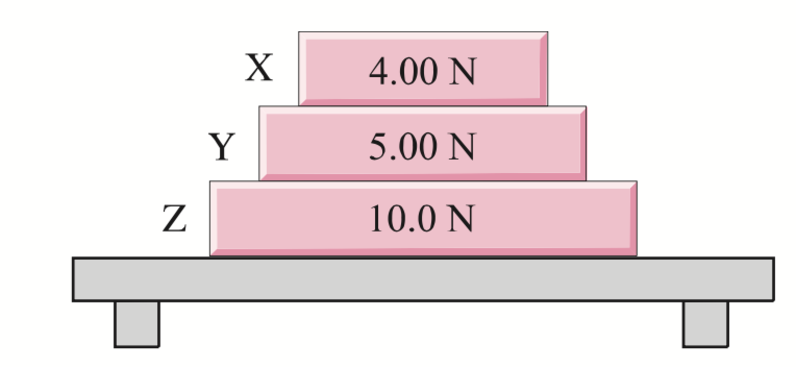
\includegraphics[scale=0.6]{Qfig5-1.pdf}  
  \caption{문제 1}
  \label{fig:1}
\end{figure}

\noindent {\bf 해답}
책 Y 는 정지해 있으므로, 책 Y 에 작용하는 알짜힘은 0 N 이다.

\vspace{2cm}

\noindent {\bf 문제 2 [10pt]}
화물이 실린 어떤 비행기의 무게는 $2.75\times
10^6$ N이다. 이 비행기의 엔진 추진력이 $6.35\times10^6$ N이라면 최저
이륙속력인 285 km/h에 도달하기 위해 필요한 활주로의 길이는 최소
얼마인가?  \\

\noindent {\bf 해답} 비행기의 무게를 $W$, 질량을 $m$ 이라 하자. 
무게는 비행기의 질량에 중력 가속도의 크기를
곱한 값과 같으므로,
\begin{align}
  W=mg,\,\,\,m=\frac{W}{g}.
\end{align}
비행기가 엔진에 의해 가속될 때, 엔진의 추진력을 $F$ 라 하면 
그 가속도의 크기는 다음과 같이 일정하다.
\begin{align}
  a=\frac{F}{m}=\frac{Fg}{W}
\end{align}
비행기가 일정한 가속도로 질주하므로 질주한 거리와 그 때의 속력은 
다음의 식을 통해 구할 수 있다.
\begin{align}\label{eq:1}
 v^2-v^2_0 = 2a(x-x_0) 
\end{align}
초기 조건이 $x_0=0,\,\,\,v_0=0$ 로 주어진다면, 식 (\ref{eq:1}) 으로
부터 속력이 285 km/h 에 도달할 때까지 질주한 거리를 알 수 있다.
\begin{align}
    v^2 = 2ax = 2\,\frac{Fg}{W}\,x,\,\,\,
    x=\frac{2Wv^2}{Fg}
\end{align}
질주한 거리는 다음과 같다.
\begin{align}
  \begin{split}
    x&=\frac{2Wv^2}{Fg}
    =\frac{2(2.75\times 10^6\,\mathrm{N}){(285\,\mathrm{km/h})}^2}
    {(6.35\times 10^6\,\mathrm{N})(9.80\,\mathrm{m/s^2})}
    \left(\frac{1000\,\mathrm{m}}{1\,\mathrm{km}}\right)
    \left(\frac{1\,\mathrm{h}}{3600\,\mathrm{s}}\right)^2 \\
    &=\frac{(7180)(1000)}{(3600)^2}\,\mathrm{km}  \\
    &=0.554\,\mathrm{km} \\
    &= 554\,\mathrm{m}
  \end{split}
\end{align}
비행기가 질주한 거리 즉, 최저 이륙속력에 도달하기 위해 필요한 
활주로의 길이는 554 m 이다.
%{(285\,\mathrm{km/h})}^2

\vspace{2cm}

\noindent {\bf 문제 3 [15pt]}
 그림~\ref{fig:3}에서처럼 쓸림이 없는 식탁 위에 레몬이 놓여있다. 이
 레몬에 가해지는, 수평 방향의 힘 세 개 힘 중에서  두 개 $\vec{F}_1$,
 $\vec{F}_2$가 표시되어 있다. 힘 $\vec{F}_1$의 크기는 6.00 N이고,
$\theta_1=30.0^\circ$, $\vec{F}_2$의 크기는 7.00 N,
$\theta_2=30.0^\circ$이다. 
\begin{figure}[ht]
  \centering
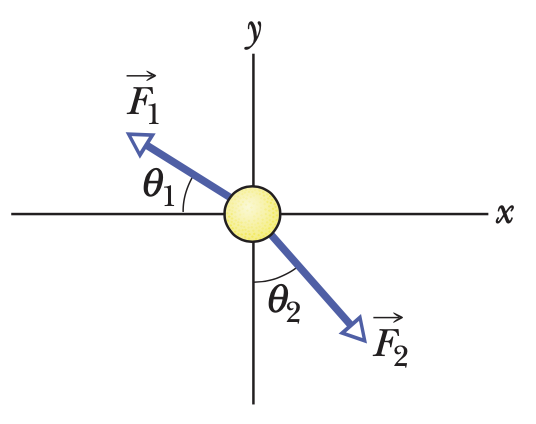
\includegraphics[scale=0.6]{Qfig6-3-20220316.png}  
  \caption{문제 3}
  \label{fig:3}
\end{figure}
\begin{itemize}
\item[(가)] 레몬이 정지해 있으려면,
\item[(나)] 레몬이 일정한 속도 $\vec{v} =(13.0\,\hat{\bm{i}} -
  14.0\,\hat{\bm{j}})\,\mathrm{m/s}$로 움직이려면, 
\item[(다)] 레몬이 속도 $\vec{v} =(13.0t\,\hat{\bm{i}} -
  14.0t\,\hat{\bm{j}})\,\mathrm{m/s}$로 움직이려면, 
\end{itemize}
세 번째 힘은 어떻게 주어져야 하는가? 각각의 경우에 힘을 단위벡터로
표현하여 나타내어라. \\ \\

\noindent {\bf 해답}
\begin{itemize}
  \item[(가)] 레몬이 정지해 있기 위해서는 레몬에 작용하는 알짜힘이
  0 N 이어야 한다. 정지해 있는 레몬에 작용하는 알짜힘은 다음과 같다.
  \begin{align}
    \sum\vec{F}=\vec{F}_1 + \vec{F}_2 + \vec{F}_3 = \vec{0}
  \end{align}
  알짜힘의 $x$ 성분과 $y$ 성분은 각각 0 이다.
  \begin{align}
    \begin{split}
      \sum F_x = {F_1}_x + {F_2}_x + {F_3}_x = 0  \\
      \sum F_y = {F_1}_y + {F_2}_y + {F_3}_y = 0  
    \end{split}
  \end{align}
  $\vec{F}_1$ 과 $\vec{F}_2$ 는 + $x$ 축을 기준으로 각각
  $180^\circ-\theta_1$ , $270^\circ+\theta_2$ 만큼 벌어져 있으므로
  삼각함수의 성질에 따라
  $x$ 성분과 $y$ 성분을 다음과 같이 구할 수 있다.
  \begin{align}
    \begin{split}
      {F_1}_x + {F_2}_x + {F_3}_x 
      &= |\vec{F}_1|\cos{(180^\circ-\theta_1)}
      +|\vec{F}_2|\cos{(270^\circ+\theta_2)} + {F_3}_x  \\
      &=-|\vec{F}_1|\cos{\theta_1}
      +|\vec{F}_2|\sin{\theta_2} + {F_3}_x = 0  \\
    \end{split}  
  \end{align}
  \begin{align}
    \begin{split}
      {F_1}_y + {F_2}_y + {F_3}_y 
      &= |\vec{F}_1|\sin{(180^\circ-\theta_1)}
      +|\vec{F}_2|\sin{(270^\circ+\theta_2)} + {F_3}_y  \\
      &= |\vec{F}_1|\sin{\theta_1}
      -|\vec{F}_2|\cos{\theta_2} + {F_3}_y=0
    \end{split}
  \end{align}
  따라서, ${F_3}_x$ 와 ${F_3}_y$ 는 다음과 같다.
  \begin{align}
    \begin{split}
      {F_3}_x&=|\vec{F}_1|\cos{\theta_1}-|\vec{F}_2|\sin{\theta_2} 
      =6\cos{30.0^\circ}-7\sin{30.0^\circ}  \\
      &=\frac{6\sqrt{3}}{2}-\frac{7}{2} = 1.70 
    \end{split}
  \end{align}
  \begin{align}
    \begin{split}
      {F_3}_y&=-|\vec{F}_1|\sin{\theta_1}+|\vec{F}_2|\cos{\theta_2}
      =-6\sin{30.0^\circ}+7\cos{30.0^\circ}   \\
      &=-\frac{6}{2}+\frac{7\sqrt{3}}{2} = 3.06
    \end{split}
  \end{align}
  $\vec{F_3}$을 단위벡터로 표현하면 다음과 같다.
  \begin{align}\label{eq:2}
    \vec{F_3}=(1.70\,\hat{\bm{i}} +
    3.06\,\hat{\bm{j}})\,\mathrm{N}
  \end{align}
  \item[(나)] 레몬이 일정한 속도 $\vec{v} =(13.0\,\hat{\bm{i}} -
  14.0\,\hat{\bm{j}})\,\mathrm{m/s}$로 움직일 때 레몬의
  가속도는 다음과 같다.
  \begin{align}
    \vec{a} = \frac{1}{m}\sum\vec{F}=\frac{d\vec{v}}{dt} = 0
  \end{align}
  즉, 알짜힘은 $\vec{0}$ 이고, 이는 정지해 있는 경우와 같다.
  따라서, 일정한 속도로 움직이기 위해 세 번째 힘은 
  다음과 같이 주어져야 한다.
  \begin{align}
    \vec{F_3}=(1.70\,\hat{\bm{i}} +
    3.06\,\hat{\bm{j}})\,\mathrm{N}
  \end{align}
  \item[(다)] 레몬이 속도 $\vec{v} =(13.0t\,\hat{\bm{i}} -
  14.0t\,\hat{\bm{j}})\,\mathrm{m/s}$로 움직일 때, $m$ 을 레몬의 
  질량이라고 하면 레몬의 가속도와 레몬에 가해지는 알짜힘은 다음과 같다.
  \begin{align}
    \vec{a} = \frac{d\vec{v}}{dt} = (13.0\,\hat{\bm{i}} -
    14.0\,\hat{\bm{j}})\,\mathrm{m/s^2},\,\,\,
    \sum\vec{F}=m\vec{a} =m(13.0\,\hat{\bm{i}} -
    14.0\,\hat{\bm{j}})\,\mathrm{N}
  \end{align}
  따라서, $\vec{v} =(13.0t\,\hat{\bm{i}} -
  14.0t\,\hat{\bm{j}})\,\mathrm{m/s}$로 움직일 때 레몬에 가해지는 알짜힘은
  다음과 같다.
  \begin{align}
    \sum\vec{F} = \vec{F_1}+\vec{F_2}+\vec{F_3} 
    = m(13.0\,\hat{\bm{i}} - 14.0\,\hat{\bm{j}})\,\mathrm{N}
  \end{align}
  식 (\ref{eq:2}) 에 의해,
  \begin{align}
    \vec{F_1}+\vec{F_2} = -(1.70\,\hat{\bm{i}} +
    3.06\,\hat{\bm{j}})\,\mathrm{N}.
  \end{align}
  최종적으로, $\vec{F_3}$ 는 다음과 같다.
  \begin{align}
    \begin{split}
      \vec{F_3} &= -(\vec{F_1}+\vec{F_2})
      +m(13.0\,\hat{\bm{i}} -14.0\,\hat{\bm{j}})\,\mathrm{N}  \\
      &= (1.70\,\hat{\bm{i}} +3.06\,\hat{\bm{j}})\,\mathrm{N}
      +m(13.0\,\hat{\bm{i}} -14.0\,\hat{\bm{j}})\,\mathrm{N}  \\
      &=((1.70+13.0m)\,\hat{\bm{i}}+(3.06-14.0m)\,\hat{\bm{j}})\,\mathrm{N}
    \end{split}
  \end{align}
\end{itemize}
\vspace{2cm}

\noindent {\bf 문제 4 [15pt]}
질량이 $1.0\times 10^{-4}$ kg인 공이 줄에 매달려 있다. 수평방향으로
불어오는 일정한 세기의 산들바람이 공을 밀어 줄이 수직과 $45^\circ$를
이루었다.
\begin{itemize}
\item[(가)] 미는 힘의 크기를 구하여라.
\item[(나)] 줄의 장력을 구하여라.
\end{itemize}

\noindent {\bf 해답}
\begin{itemize}
  \item[(가)]
  산들바람이 공을 미는 힘을 $\vec{D}$, 공에 작용하는 중력을
  $\vec{W}$ 그리고 공에 작용하는 장력을 $\vec{T}$ 라 하자.
  $\vec{W}$ 는 다음과 같다.
  \begin{align}
    \vec{W} = m\vec{g} 
    = -(1.0\times 10^{-4}\,\mathrm{kg})(9.80\,\mathrm{m/s^2})\,\hat{\bm{j}}
  \end{align}
  공은 정지해 있으므로, 공에 작용하는 알짜힘은 $\vec{0}$ 이다.
  \begin{align}\label{eq:3}
    \sum\vec{F}=\vec{W}+\vec{D}+\vec{T} = \vec{0}
  \end{align}
공에 작용하는 알짜힘의 성분은 다음과 같다.
\begin{align}\label{eq:4}
  \begin{split}
    F_x &= |\vec{D}|-|\vec{T}|\cos{45^{\circ}} \\
    &= |\vec{D}|-\frac{\sqrt{2}}{2}|\vec{T}|
    = 0   
  \end{split}
\end{align}
\begin{align}\label{eq:5}
  \begin{split}
    F_y &= |\vec{W}|-|\vec{T}|\sin{45^{\circ}}  \\
    &= (1.0\times 10^{-4}\,\mathrm{kg})(9.80\,\mathrm{m/s^2})
    -\frac{\sqrt{2}}{2}|\vec{T}|
    = 0
  \end{split}
\end{align}
식 (\ref{eq:4}) 와 식 (\ref{eq:5}) 에 의해,
\begin{align}
  \begin{split}
    |\vec{D}| &= \frac{\sqrt{2}}{2}|\vec{T}|
    = (1.0\times 10^{-4}\,\mathrm{kg})(9.80\,\mathrm{m/s^2})  \\
    &=9.8\times 10^{-4}\,\mathrm{N}.
  \end{split}
\end{align}
미는 힘의 크기는 $9.8\times 10^{-4}\,\mathrm{N}$ 이다.
\item[(나)] 식 (\ref{eq:3}) 에 의해 줄의 장력 $\vec{T}$ 는 다음과 같다.
\begin{align}
  \vec{T} = -\vec{D}-\vec{W}
\end{align}
$\vec{D}$ 는 수평 방향으로만 작용하므로 단위벡터로 표현하면 다음과 같다.
\begin{align}
  \vec{D} = (9.8\times 10^{-4}\,\hat{\bm{i}})\,\mathrm{N}
\end{align}
따라서, 장력 $\vec{T}$ 는 다음과 같다.
\begin{align}
  \begin{split}
    \vec{T} &= -\vec{D}-\vec{W} \\
    &=-(9.8\times 10^{-4}\,\hat{\bm{i}})\,\mathrm{N}
    +(9.8\times 10^{-4}\,\hat{\bm{j}})\,\mathrm{N}  \\
    &=(-9.8\times 10^{-4}\,\hat{\bm{i}}
    +9.8\times 10^{-4}\,\hat{\bm{j}})\,\mathrm{N}
  \end{split}
\end{align}

\begin{figure}[ht]
  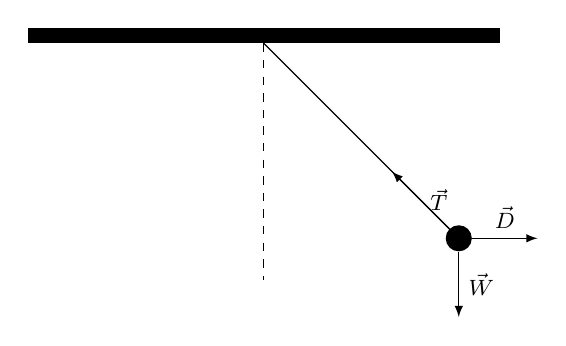
\begin{tikzpicture}[font=\footnotesize]

    % Support
    \fill (-3,0) rectangle(3,0.2);
    
    % Bob's trajectory
    \draw[dashed] (0,0) -- (0,-3) ;
    % Rod + Bob
    \draw (0,0) -- (-45:3.5) node[fill,circle](m){};
    
    % Weight Force
    \draw[-latex] (m) -- node[right]{$\vec{W}$}++(0,-1) ;

    \draw[-latex] (m) -- node[right,above]{$\vec{D}$}++(1,0) ;
    % Tension Force
    \draw[-latex] (m) -- node[right]{$\vec{T}$}(-45:2.3);

    \end{tikzpicture}
    \caption{문제 4} 
    \label{fig:4}
  \end{figure}
\end{itemize}
\end{document}